\documentclass[11pt,a4paper]{article}

\usepackage[utf8]{inputenc}
\usepackage{times}
\usepackage[left=2cm,top=3cm,text={17cm, 24cm}]{geometry}

\usepackage{graphicx}
\usepackage{setspace}
\usepackage{hyperref}
\usepackage{multirow}
\usepackage{pdflscape}
\usepackage{url}
\DeclareUrlCommand\urlmoje{\urlstyle{tt}}
\bibliographystyle{czplain}

\begin{document}

    \begin{titlepage}
    \begin{center}
      {\Huge
      \textsc{Vysoké učení technické v~Brně} \\
      \medskip
		\huge{\textsc{Fakulta informačních technologií}}
       }\\
      %\vspace{\stretch{0.191}}
      \begin{figure}[h]
		\begin{center}
		\scalebox{0.8}{
\includegraphics{fit.png}}
		\end{center}
	  \end{figure}
	  %\vspace{\stretch{0.191}}
      {\LARGE
      Dokumentace k projektu do předmětů IFJ a IAL}\\
      \LARGE{\textbf{Implementace překladače imperativního jazyka IFJ17}}
      \vspace{\stretch{0.060}}
      
      {\LARGE Tým 065, varianta I}
      
      {\LARGE 31. března 2017}
      \vspace{\stretch{0.618}}
      
      {\LARGE Seznam autorů:\\}
      {\Large\itshape Vedoucí: Bártl Roman (xbartl06) - 25\%\par}
        {\Large\itshape Bartošek Jan (xbarto92) - 25\%\par}
        {\Large\itshape Odehnal Tomáš (xodehn08) - 25\%\par}
        {\Large\itshape Šopf Petr (xsopfp00) - 25\%\par}
        \vspace{\stretch{0.718}}
        {\Large \textbf{Rozšíření:} UNARY, BASE, IFTHEN}
        \vspace{\stretch{0.2}}
    \end{center}
\end{titlepage}
    
    \doublespacing
	\tableofcontents
	\singlespacing
    \newpage

\addtocontents{toc}{\setcounter{tocdepth}{3}}
\section{Scanner}
Implementoval xbarto92

	\subsection{Postup implementace}
	Při prvním návrhu lexikální analýzy jsem se inspiroval ukázkovým příkladem, kde byl scanner řešený s využitím přepínače switch umístěného v nekonečné smyčce. První verze scanneru spatřila světlo světa již 7. října, ovšem její funkčnost byla naprosto nevyhovující, a tak jsem scanner postupně opravoval a rozšiřoval.
	
	Původní verze scanneru vracela pouze integer hodnotu, která reprezentovala přečtený lexém a nedokázala rozlišovat klíčová slova od identifikátorů. Tento problém jsem vyřešil vytvořením pole, jehož hodnoty odpovídají všem rezervovaným klíčovým slovům a v případě zjištění identifikátoru, pak jeho porovnáním.
	
	Následovalo vytvoření struktury reprezentující token nesoucí informace o typu přečteného lexému (číslo, ID, atd..), jeho hodnotu (např.: název proměnné) a v poslední řadě zde byla přidána i hodnota řádku, která slouží pro výpis chybových hlášek a lepší debug. Dřívější myšlenka byla taková, že scanner by měl hodnotu přečteného tokenu hned zapsat do tabulky symbolů. Z tohoto důvodu jsem připravil binární strom a dynamický stack, právě pro práci s touto tabulkou. Nicméně po delší úvaze jsme se rozhodli zanechat tuto úlohu mimo parser, a tak se jejím vyřešením zaobírali mí kolegové.
	
	V momentě, kdy scanner již obstojně interpretoval jakýkoliv příchozí lexém jsem se začal zaobírat rozšířeními UNARY a BASE, kde první z nich jsem jako speciální token posílal ke zpracování parseru, a ten druhý nahrál a funkcí strtol převedl hodnotu čísla do dekadické soustavy a posílal jako jakékoli jiné číslo. V neposlední řadě jsem se zaobíral testováním všech možných chybových stavů a jejich správným řešením.

	\subsection{Funkce}
	Lexikální analýza implementovaná v souborech scanner.c a scanner.h cyklicky načítá ze vstupu znak po znaku a každý ihned interpretuje a kontroluje jejich vzájemnou návaznost.
	
	Funkce getNextToken(), která obstarává celou lexikální analýzu, se volá v parseru při potřebě následujícího tokenu. Při správné posloupnosti znaků je vrácen token, neboli struktura, která se skládá ze tří hodnot (viz výše). V opačném případě se na chybový výstup vypíše odpovídající chybová hláška spolu s řádkem v kódu, na kterém k chybě došlo.
    \newpage

\subsection{Konečný Automat Lexikální Analýzy}
\vspace{1cm}
	\centerline{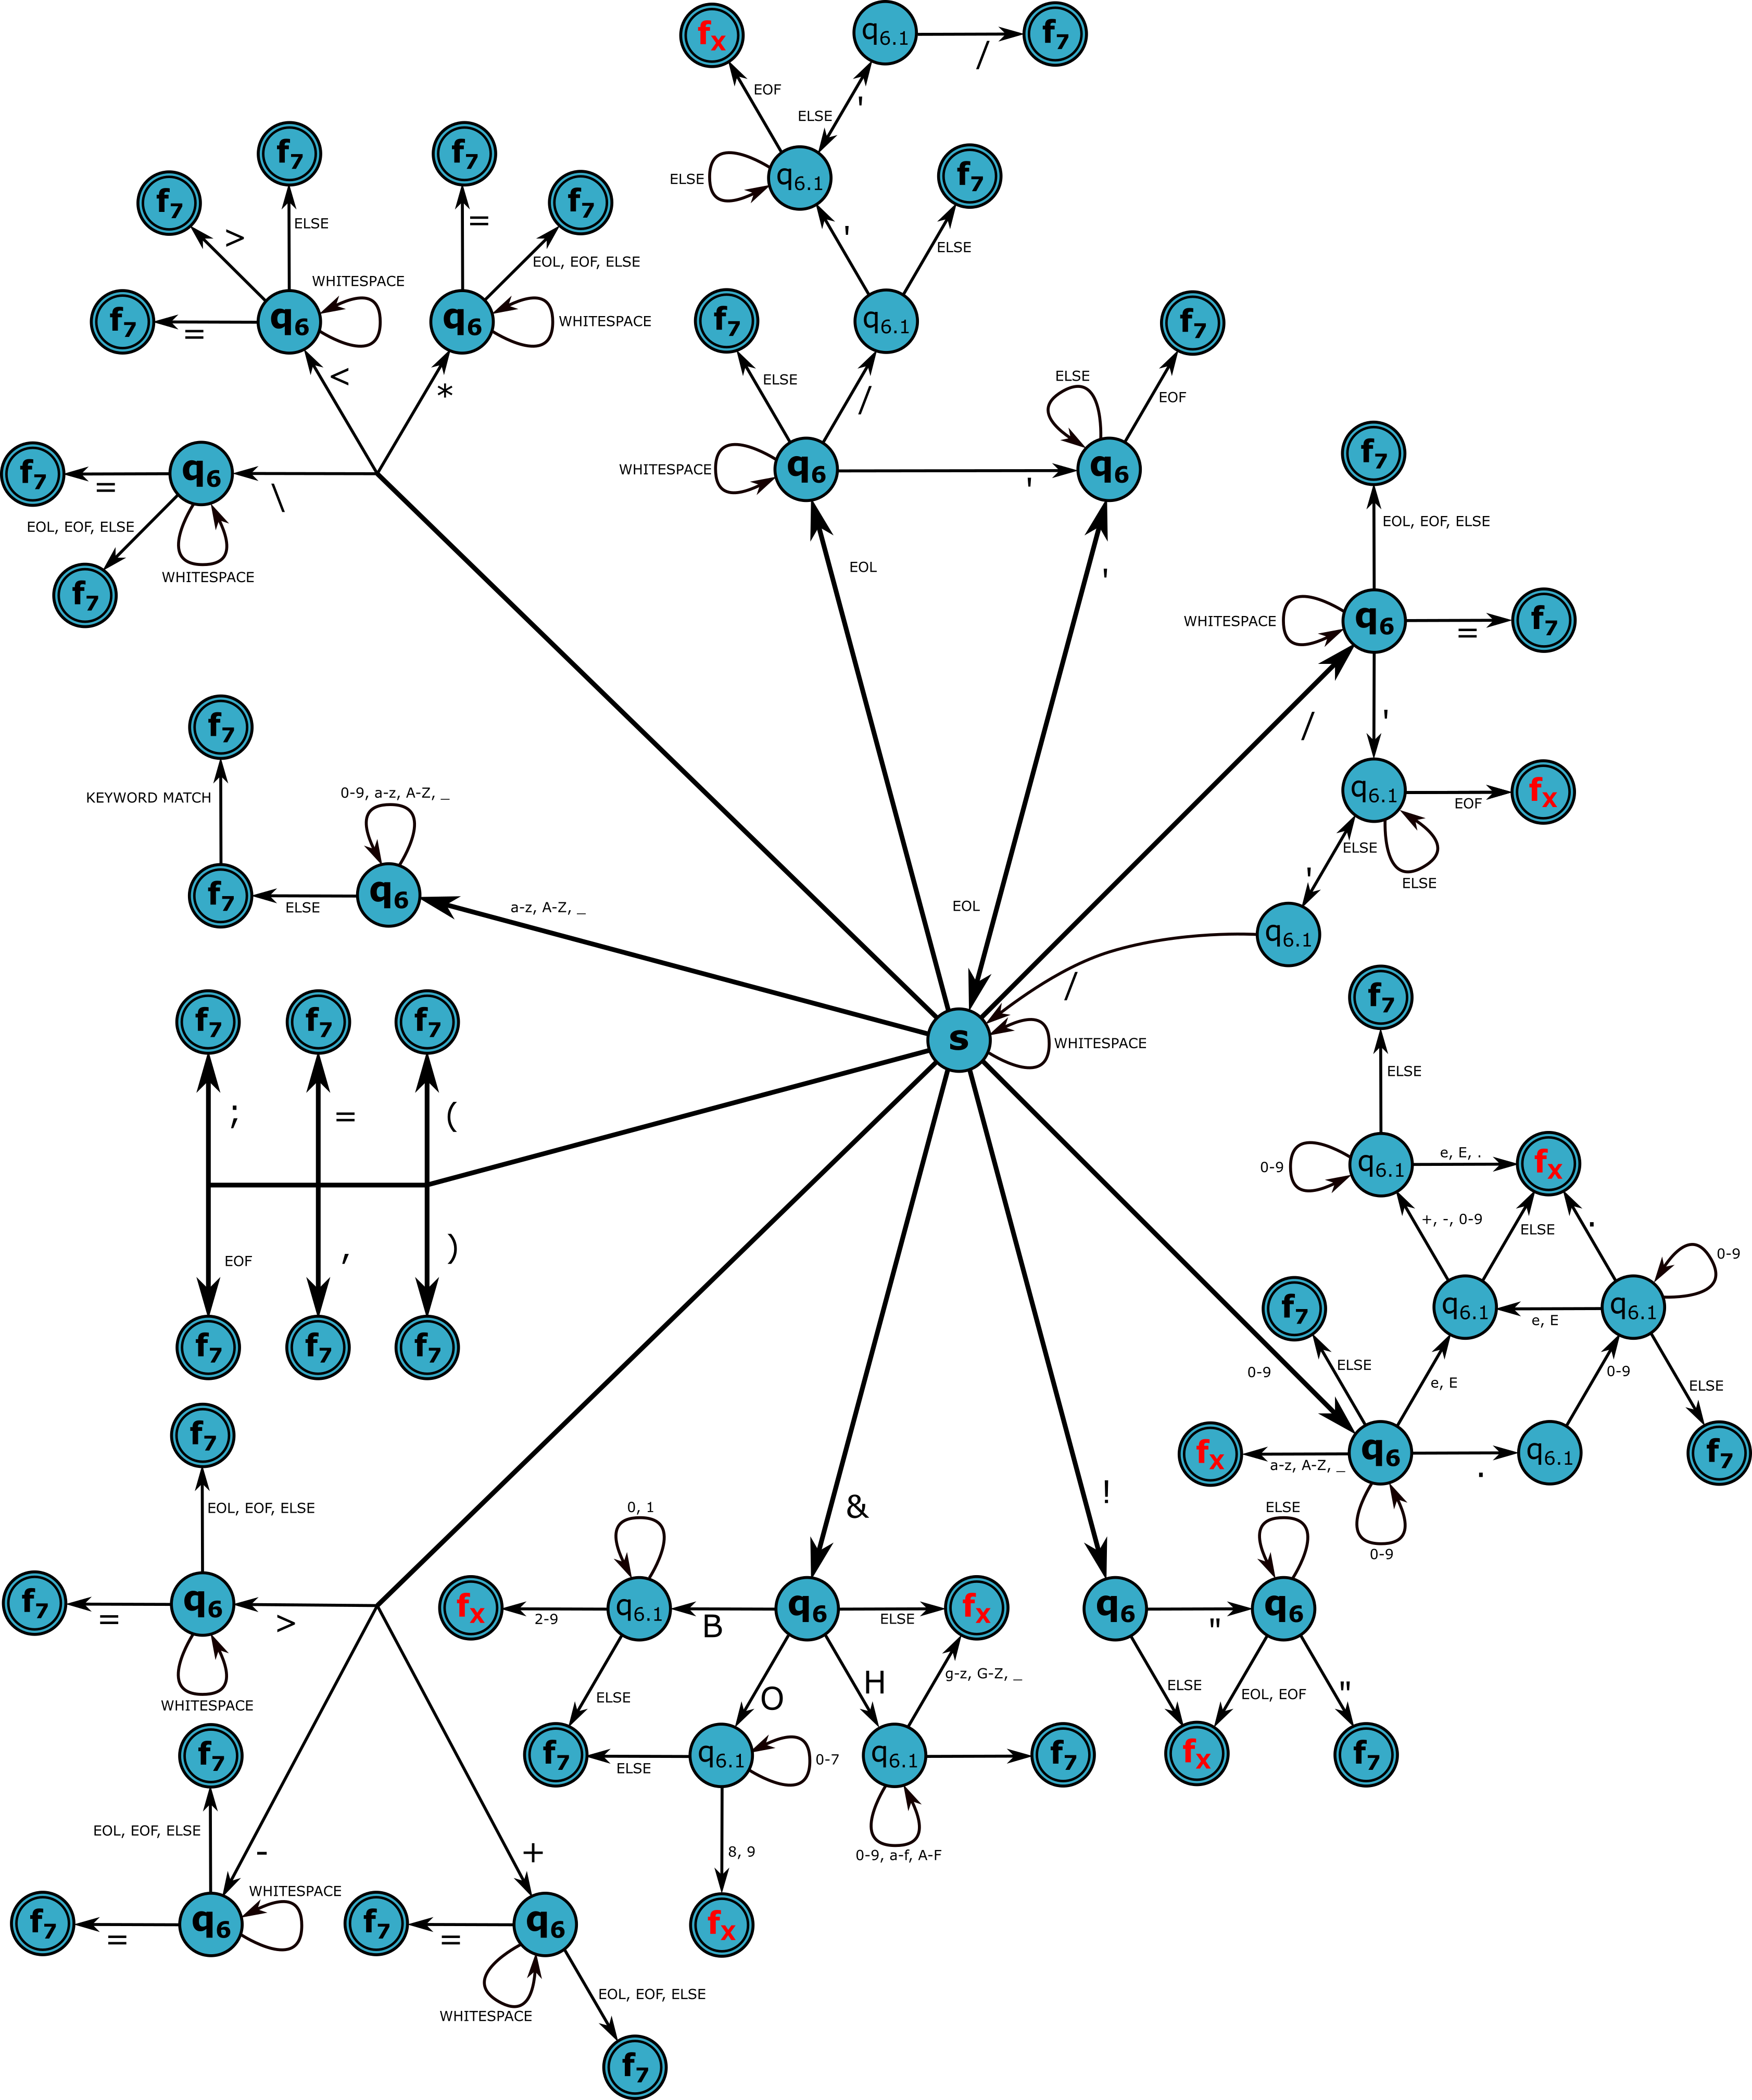
\includegraphics[height=21cm]{KA.png}}
    {\newpage}



\section{Parser - Syntax}
    Implementoval xbartl06

    \subsection{Postup implementace}
    Před samotnou implementací syntaktické anaylýzy bylo zapotřebí sestavit LL-gramatiku určující pravidla jazyka IFJ17 (viz kapitola \ref{LL_Gramatika}) a precedenční tabulku pro zpracovávání výrazů (viz kapitola \ref{LL_Tabulka}).

    


    \subsubsection{LL-gramatika} \label{LL_Gramatika}

    \subsubsection{LL-tabulka} \label{LL_Tabulka}

    \subsection{Funkce}


    \newpage



\section{Parser - Sémantika}
    Implementoval xodehn08

    \subsection{Funkce}
    Sémantická analýza ověřuje sémantickou správnost zpracovávaného zdrojového kódu. V našem projektu je výstupem sémantické analýzy (tedy i parseru) Abstraktní syntaktický strom (AST), který je vstupem do generátoru cílového kódu. 

    \subsection{Postup Implementace}
    Během syntaktické analýzy (práce parseru), který simuluje konstrukci derivačního stromu, probíhala i částečná sémantická analýza a zbytek u generování kódu. V parseru šli řešit sémantické akce typu: nedeklarované / nedefinované funkce a proměnné, špatný počet a datové typy parametrů funkcí, neslučitelné datové typy ve výrazech, atd. Těchto sémantických kontrol (akcí) lze dosáhnout použitím tabulky symbolů. V generátoru kódu se provádí např. implicitní konverze ve výrazech nebo kontrola dělení nulou.
    
    Implementace probíhala tak, že jakmile byl parser z větší části implementovaný, začal se do něj dopisovat kód pro provádění sémantických akcí.
    
    \subsection{Tabulka symbolů}
    Náš tým měl první variantu projektu. Tabulka symbolů se tedy implementovala jako binární vyhledávací strom. Do této tabulky symbolů si ukládáme vše, co potřebujeme např. jestli je uzel stromu proměnná nebo funkce, dále definice / deklarace proměnných a funkcí. U funkcí si dále ukládáme počet a datové typy parametrů a návratové hodnoty. U každé funkce si vytváříme "menší" tabulku symbolů, do které se ukládají lokální proměnné (i parametry dané funkce).
    
    Do tabulky symbolů si neukládáme vestavěné funkce, které jsou implementované v generátoru kódu. Informace o nich jsou uloženy v samostatném poli, které se využije při kontrole volání funkce.
    
    \subsection{Abstraktní syntaktický strom}
    Součástí sémantiky je i vytvoření abstraktního syntaktického stromu (dále jen AST). Stejně jako sémantické akce i naplňování AST probíhá zároveň s prací parseru.
    
    AST je reprezentováno jako globální pole, které se postupně naplňuje uzly AST reprezentující příkazy. Příkazy a výrazy jsou reprezentovány dvěma strukturami. Přesný typ výrazu / příkazu je určen "tagem" a "op". "Op" je prvek typu union, který obsahuje struktury reprezentující konkrétní příkaz / výraz. Pro určení, se kterou strukturou z prvku "op" se pracuje, slouží prvek "tag", který je typu enum. Uzel AST pro výraz navíc obsahuje prvek "datatype" určující datový typ daného uzlu (výrazu). \cite{AST:AST_in_C}
    
	\newpage


\section{Generátor}
    Implementoval xsopfp00

    \subsection{Postup implementace}
    \noindent Hinzufügen den Text hier!

    \subsection{Funkce}
    \noindent Hinzufügen den Text hier!

    \newpage
    \bibliography{dokumentace}
\end{document}